\section{What to change, and what it costs}
\label{sec:mitigation}

The factors in Sec.~\ref{sec:controlled} are choices made before training, so they translate
directly into settings. Each recommendation is stated with the measurement behind it and with its
cost, ordered by the size of the lever: the objective removes verbatim extraction, the tokeniser
only postpones it. Table~\ref{tab:mitigation} collects them, and every cell in it is a
measurement from this paper rather than an expectation.

\paragraph{Prefer a masked objective wherever generative output is not needed.}
This is the one setting that removes verbatim extraction rather than delaying it, and on our
measurements it costs nothing. With the backbone, the data and the 30-round schedule fixed and the
planted records being real human haplotype segments, a masked objective memorises
\NUM{15}--\NUM{35}$\times$ less than the same tokeniser trained next-token and reproduces no segment
at any snapshot: \excess{} falls from \NUM{4.27} to \NUM{0.12} for the \kmer{3} and from \NUM{2.45}
to \NUM{0.16} for the \kmer{6}, with extraction from \NUM{100\%} to \NUM{0\%} in every case, and the
masked cells reach a \emph{better} held-out loss on the same budget (\NUM{1.67}--\NUM{1.85} against
\NUM{2.35}--\NUM{3.93}~\bits). Across all five datasets no masked cell reproduces anything
(Fig.~\ref{fig:objaxis}). It is not confined to our backbone: fine-tuning the released DNABERT
checkpoints under their own masked objective at matched hidden-nucleotide rate on chromosome~22
leaves \excess{} at \NUM{0.58}--\NUM{1.05} with \NUM{0\%} extraction ($\kmer{6}$: \NUM{10\%}),
against \NUM{1.43}--\NUM{1.54} and \NUM{67}--\NUM{97\%} for the same checkpoints fine-tuned
next-token. \textbf{The cost is categorical rather than quantitative}: a masked model cannot be
sampled from, so this does not apply to generative uses --- but it does apply to the embedding and
classification uses that most genomic pipelines need, which is where the released encoder-only
models are actually used. One caveat for anyone measuring this: with overlapping $k$-mers a
\NUM{15\%} \emph{token} mask hides only $15/k$ per cent of the \emph{nucleotides}, so a masked
$k$-mer model looks safer than it is unless the comparison is at matched hidden-nucleotide rate.

\paragraph{Asked in its own idiom, the masked model still returns nothing.}
Prefix-only probing is the weak way to ask a model that denoises arbitrary positions: on diffusion
language models, edge-conditioned masks recover up to three times more verbatim sequences
\cite{wang2026infilling}. We therefore re-ran every masked cell with the sequence after the record
left visible and the 48 masked nucleotides decoded in confidence order. Across 120 cells --- five
datasets, every tokeniser, both mask rates, two to three seeds, all three tiers, 20 canaries each ---
edge-conditioned extraction recovers no record either: \NUM{0\%} under both protocols, with
\NUM{34.9} wrong nucleotides out of 48 under the prefix protocol and \NUM{35.2} under infilling,
against \NUM{35.0}--\NUM{35.6} for non-members (Appendix~A8).

\paragraph{Tokenise finely: a delay, not immunity.}
On real human sequence, with the backbone matched and the same 30-round schedule, the onset of
leakage follows token length: first extraction at round~5 for BPE, round~8 for the \kmer{6} and
round~8--12 for the \kmer{3}, with the character cell showing none within 30 rounds. \textbf{It is a
delay, not immunity}: on an identical 150-round schedule the character cell reaches \NUM{100\%}
extraction and \NUM{11.5}--\NUM{11.8} excess bits, while the \kmer{6} is already fully extractable by
round~20 (Fig.~\ref{fig:delay}). The delay is about an order of magnitude in rounds and it cannot be
cashed in: at a matched held-out loss of \NUM{2.4}~\bits{} the \kmer{6} reproduces \NUM{100\%} of the
planted segments and the character cell \NUM{30\%}, and by the time the character cell reaches
\NUM{100\%} its held-out loss has degraded to \NUM{10.2}~\bits. The cost is compute: 96 token slots
per window against 16.

\begin{figure}[t]
\centering
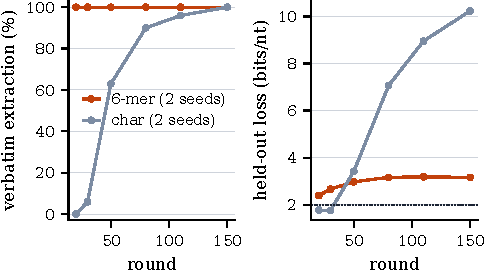
\includegraphics[width=0.49\textwidth]{figures/F4_delay.pdf}
\caption{Fine tokenisation postpones extraction, it does not prevent it. Real human canaries, an
identical 150-round schedule, two seeds each. \textbf{Left:} the \kmer{6} reproduces every planted
record from round~20; the character cell reaches \NUM{0\%}, \NUM{63\%} and \NUM{100\%} at rounds 20,
50 and 150. \textbf{Right:} the price of getting there --- the character cell's held-out loss
degrades to \NUM{10.2}\,\bits{} while the \kmer{6} stays near \NUM{3.2}, so the delay cannot be
cashed in for a usable model.}
\label{fig:delay}
\end{figure}

\paragraph{Do not rely on early stopping or on downstream scores.}
Sec.~\ref{sec:utility} shows both fail: the held-out-loss optimum sits on the steep part of the
memorisation curve, one snapshot from complete reproduction, and the best downstream checkpoint is
usually the leakiest.

\paragraph{Randomise the position of records that must appear more than once.}
This one is aimed at the auditor more than the trainer. When every copy sits at the same offset, a
model with learned absolute positions can score the record from its position, and the variance
decomposition then attributes \NUM{59.5\%} of the effect to the tokeniser against \NUM{15.4\%} under
drawn offsets (Sec.~\ref{sec:controlled}). Anyone measuring memorisation should draw the offsets, or
the measurement will report a tokeniser effect that is partly position matching. As a mitigation it
is weak but free.

\paragraph{What we do not recommend here.}
Differential privacy is outside this paper's scope. Our question is what the architecture itself
contributes, and a DP comparison needs its own utility study; DP-SGD and parameter-efficient
fine-tuning are complementary to these settings rather than alternatives
(Sec.~\ref{sec:discussion}).

\begin{table}[t]
\centering
\caption{Architectural settings, their measured effect on leakage and their measured cost. This is
the table a practitioner will read; every cell is a number from this paper. Levers are ordered by
effect size, and every cell is a measurement from this paper rather than an expectation.}
\label{tab:mitigation}
\begin{tabular}{p{2.4cm}p{3.5cm}p{4.3cm}p{3.5cm}}
\toprule
lever & recommended setting & measured effect on leakage & measured cost \\
\midrule
objective & masked, wherever generative output is not required
 & extraction $100\%\!\to\!0\%$; \excess{} $15$--$35\times$ lower; holds for released checkpoints too
 & none measured: held-out loss improves ($2.35$--$3.93\!\to\!1.67$--$1.85$\,\bits), but the model
   cannot be sampled from \\
tokeniser & character level
 & delays first extraction by $\sim\!10\times$ in rounds; $100\%\!\to\!30\%$ extraction at matched
   held-out loss; not immunity ($100\%$ by round~150)
 & $6\times$ the token slots per window (96 against 16) \\
stopping rule & neither is usable as a warning: audit the checkpoint instead
 & loss optimum is $0\%$ extraction but $+0.004$--$0.111$\,\bits{} from it is $51$--$100\%$;
   best downstream score picks $44$--$100\%$ for 5 of 6 models
 & none; it removes a false sense of safety, not a capability \\
record placement & draw each copy's offset
 & fixed offsets shift $59.5\%$ of the attributed effect onto the tokeniser against $15.4\%$ when
   drawn --- mostly a measurement fix
 & none \\
\bottomrule
\end{tabular}
\end{table}
